\documentclass[preprint,12pt]{elsarticle}
\usepackage{graphicx}
\usepackage[margin=1.0in]{geometry}
\usepackage{color, colortbl}
\usepackage{hyperref}
\usepackage{float}
% \usepackage[affil-it]{authblk}
\usepackage{subcaption}
\newcommand{\note}[1]{\textcolor{blue}{#1}}
\definecolor{LightCyan}{rgb}{0.88,1,1}
\definecolor{LightRose}{rgb}{1,0.88,0.88}
\definecolor{LightGreen}{rgb}{0.88,1,0.88}

\title{Real Time Charged Track Reconstruction for CLAS12}
\author[1]{Gagik Gavalian}

% \affiliation[1]{organization={CRTC, Department of Computer Science, Old Dominion University}, city={Norfolk, VA}, country={USA}}
\address[1]{Jefferson Lab, Newport News, VA, USA}
%\address[2]{CRTC, Department of Computer Science, Old Dominion University, Norfolk, VA, USA}
%\address[3]{INFN, Sezione di Genova, 16146 Genova, Italy}

\begin{document}

%\begin{titlepage}
\begin{abstract}
In this paper, we present the results of charged particle track reconstruction in CLAS12 using artificial intelligence. In our approach, we 
use machine learning algorithms to reconstruct tracks, including their momentum and direction, with high accuracy from raw hits in CLAS12
drift chambers. The reconstruction is performed in real-time (with the rate of data acquisition) and allows to 

\end{abstract}
%\end{titlepage}
\maketitle


\section{Introduction}
\indent
Artificial Intelligence (AI) is revolutionizing the way computations are handled in nuclear physics experiments, marking a significant shift in the field. Traditionally, nuclear physics has relied on complex mathematical models and extensive computational resources to simulate and analyze experiments. These processes are often time-consuming and computationally intensive, making it challenging to quickly process large volumes of data or accurately predict outcomes in unexplored scenarios.

With the advent of AI, especially machine learning (ML) and neural networks, this paradigm is changing. AI algorithms can analyze vast datasets more efficiently than traditional methods, identifying patterns and correlations that human researchers might miss. For instance, in particle detection and identification, AI can quickly sift through millions of particle collision events to find the few that are of interest, which would be impractical with conventional computational approaches.

Furthermore, AI is enabling more accurate modeling and simulation in nuclear physics. Neural networks, trained on historical experimental data, can predict the outcomes of nuclear reactions or the behavior of subatomic particles with a high degree of accuracy. This capability is particularly useful in scenarios where experiments are either too dangerous, expensive, or technically challenging to perform.

AI is also contributing to the design of experiments and optimization of detectors. By simulating different configurations, AI can suggest the most effective experimental setups, saving time and resources. Additionally, AI is being used in the calibration of instruments and data analysis, making the process faster and more reliable.

In conclusion, AI is not just supplementing traditional computational methods in nuclear physics but is transforming the field by providing faster, more accurate, and more efficient ways to handle complex experiments. This evolution is paving the way for discoveries and advancements in nuclear physics, highlighting the growing importance of interdisciplinary approaches in scientific research.

\section{CLAS12 Detector}

The CLAS12 (CEBAF Large Acceptance Spectrometer for 12 GeV) detector is a state-of-the-art experimental apparatus used in nuclear physics research. It's located at the Thomas Jefferson National Accelerator Facility (Jefferson Lab) in Newport News, Virginia. The detector is part of an upgrade to the Continuous Electron Beam Accelerator Facility (CEBAF), which increased the maximum energy of the electron beam from 6 GeV to 12 GeV. This upgrade allows for a more in-depth exploration of the structure and properties of nucleons (protons and neutrons) and the nature of the strong force that binds them together in the atomic nucleus.


\begin{figure}[h!]
\centering
\centerline{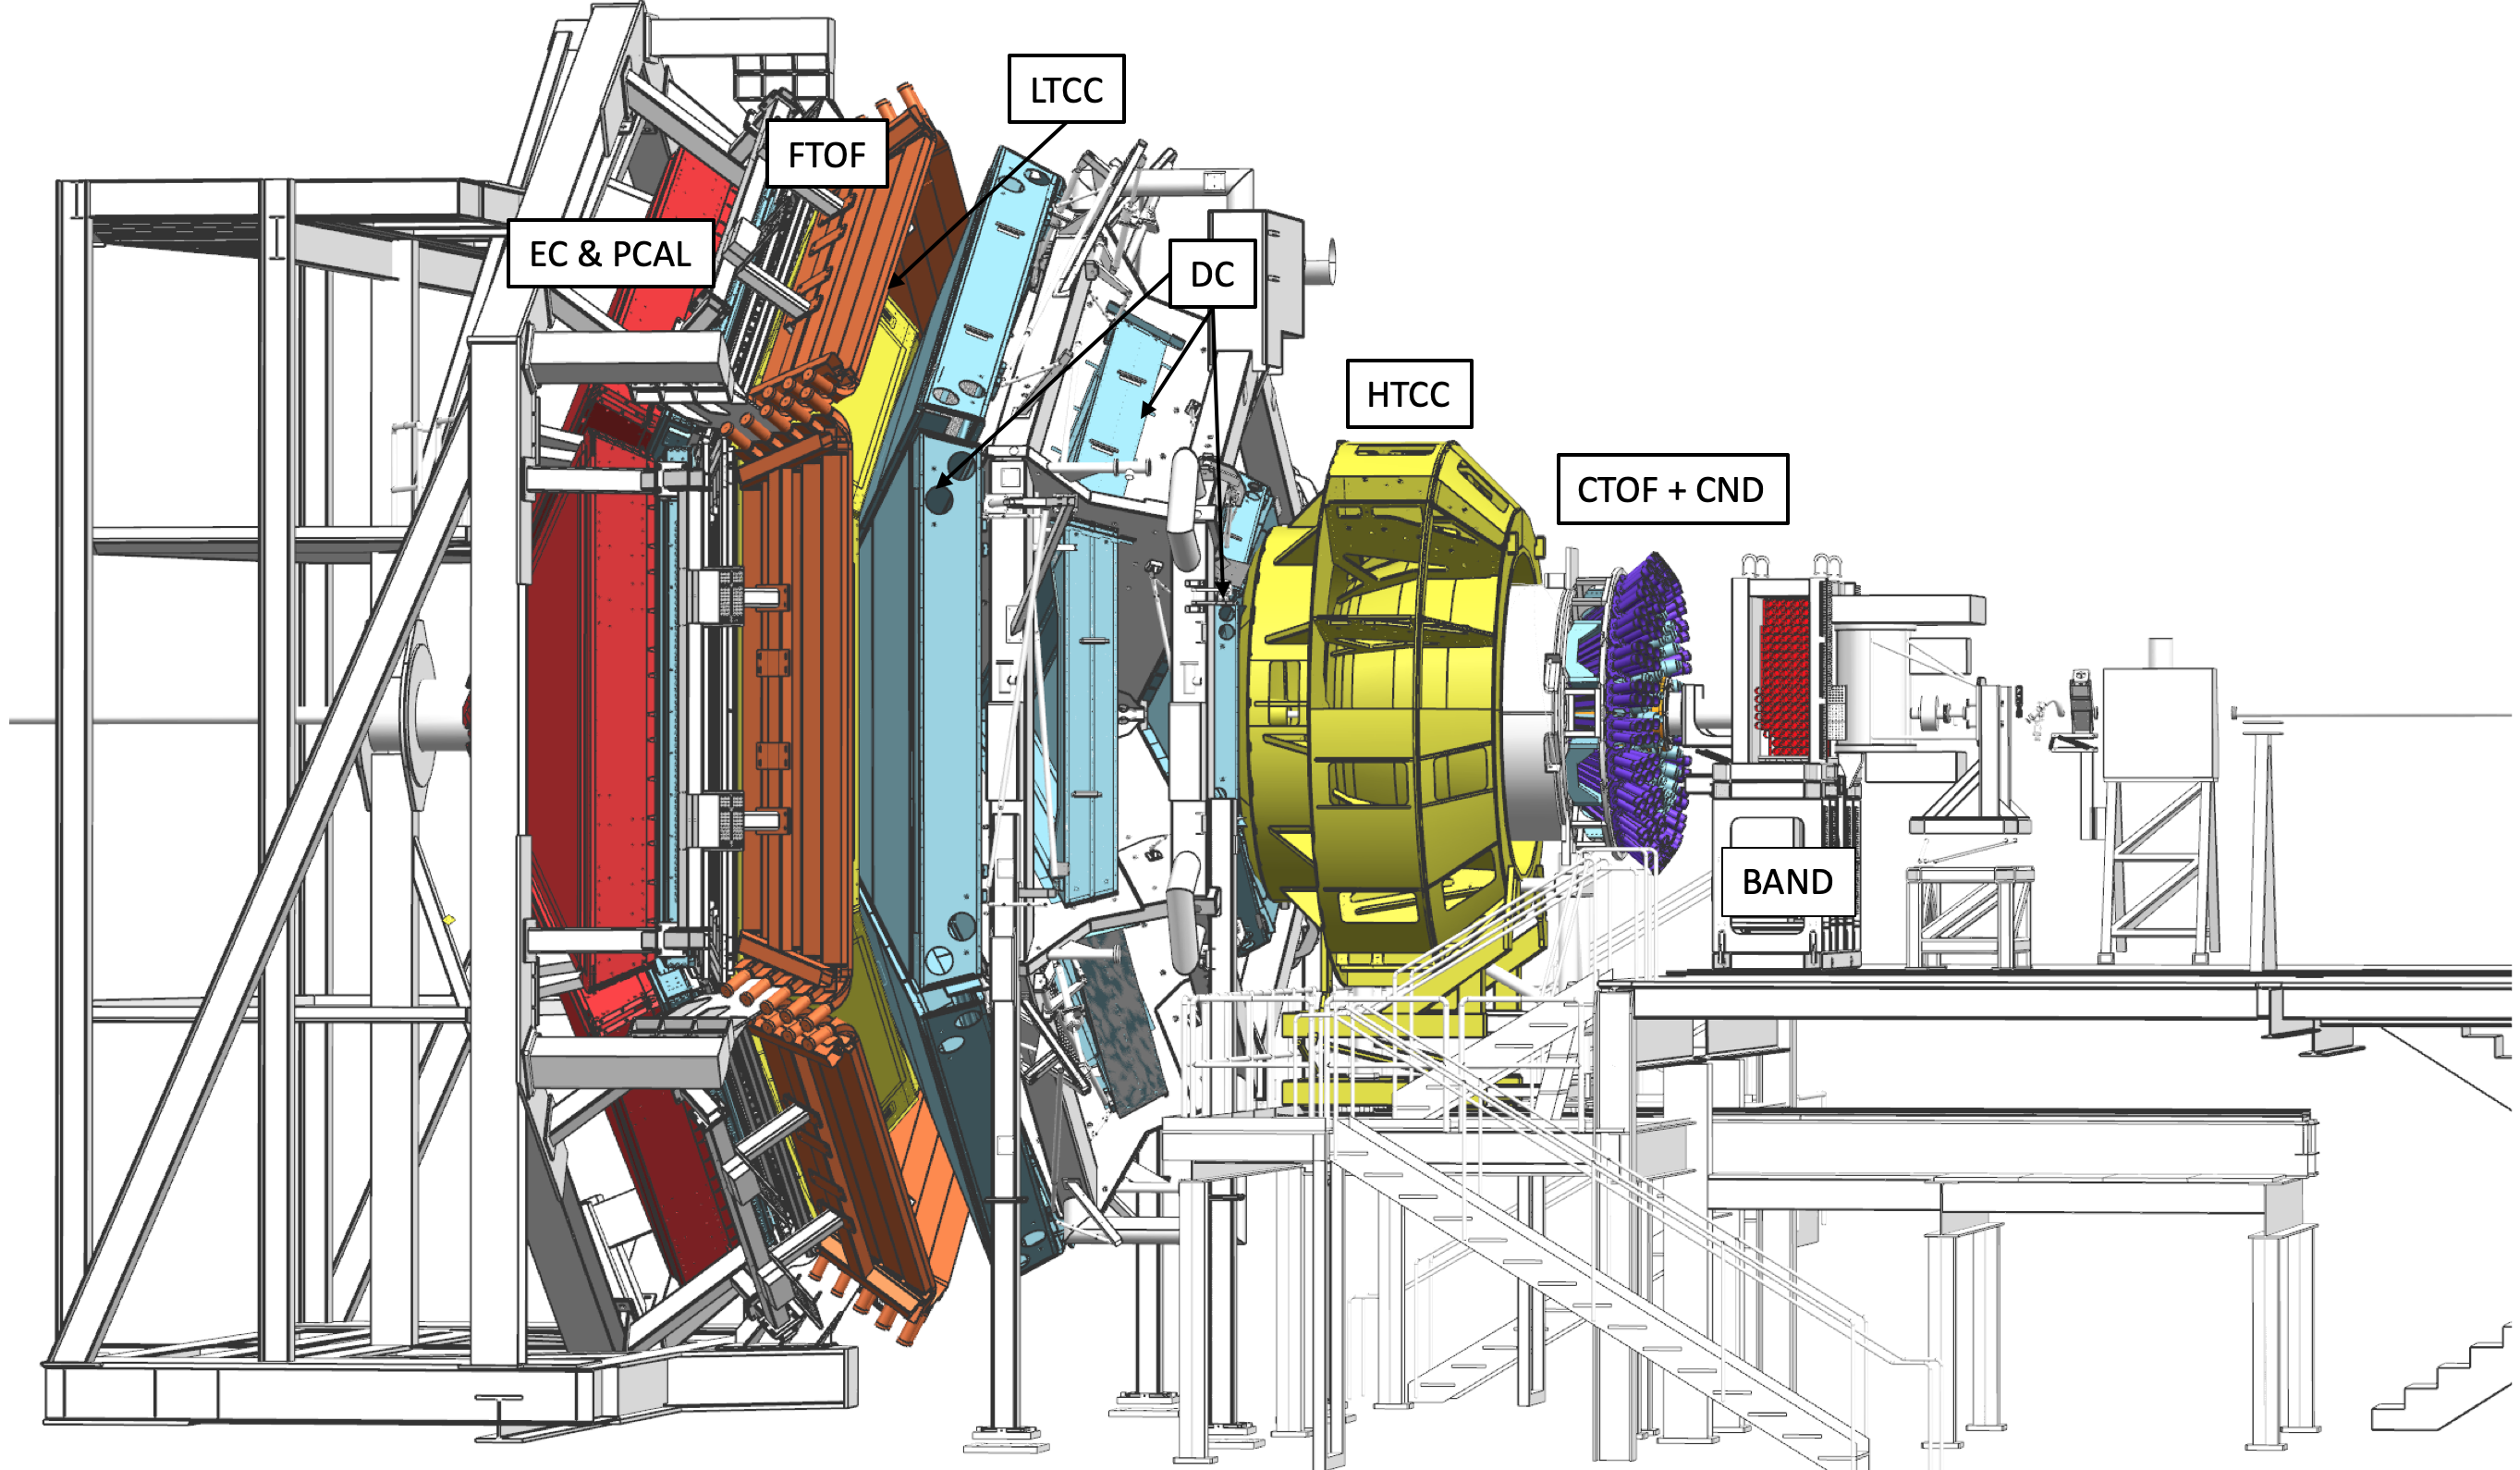
\includegraphics[width=0.7\columnwidth]{images/CLAS12-side.png}}
\caption{The CLAS12 detector in the Hall~B beamline ~\cite{Burkert:2020akg} . The electron beam enters from the right and impinges on
  the production target located in the center of the solenoid magnet shown at the right (upstream) end of CLAS12,
  where other detector components are also visible. Scattered electrons and forward-going particles are detected
  in the Forward Detector (FD), consisting of the High Threshold Cherenkov Counter (HTCC) (yellow), 
  %with full coverage in polar angle $5^\circ \le \theta \le 35^\circ$ and $\Delta \phi = 2\pi$ coverage in azimuth. The HTCC is followed
  followed by the torus magnet (gray), the drift chamber tracking system (light blue),
  and time-of-flight scintillation counters (brown), and electromagnetic calorimeters (red). 
  %Between the HTCC and the
  %torus, the Forward Tagger is installed to detect electrons and photons at polar angles $2^\circ \le \theta \le 5^\circ$.
  %The Central Detector (CD) consists of the Silicon Vertex Tracker (hidden), which is surrounded by a Barrel Micromesh
  %Tracker (hidden), the Central Time-of-Flight system, and the Central Neutron Detector (PMTs in blue). At the upstream
  %end, a Back Angle Neutron Detector (red) is installed. In the operational configuration. the entire CLAS12 detector
  %extends for 13~m along the beamline.
  } 
\label{fig:CLAS12}
\end{figure}

Key features and capabilities of the CLAS12 detector include:

\begin{itemize}

\item{\bf Large Acceptance: }As its name suggests, CLAS12 has a large angular and momentum acceptance. This feature is crucial for detecting particles over a wide range of angles and energies, allowing comprehensive analysis of nuclear reactions.
\item{\bf Electron Beam Experiments:} CLAS12 is designed to investigate the interactions of high-energy electrons with nucleons and nuclei. By scattering electrons off target materials, scientists can probe the internal structure of nucleons and the dynamics of the strong force.
\item{\bf High Luminosity:} The detector operates at high luminosities, enabling it to collect a vast amount of data from electron scattering experiments. This high data rate is essential for studying rare processes and achieving statistically significant results.
\item{\bf Sophisticated Detection Systems:} CLAS12 consists of various subsystems designed to detect different types of particles and measure their properties. These include drift chambers for tracking charged particles, time-of-flight counters for particle identification, calorimeters for measuring energy, and Cherenkov detectors for identifying electrons.
\item{\bf Versatility:} The detector is versatile and can be used for a wide range of experiments, from studying the quark-gluon structure of nucleons to investigating the properties of nuclei under extreme conditions.
\item{\bf Data Analysis and Simulation:} Advanced software and computational tools are used to analyze the data collected by CLAS12. These tools include simulation packages that model the detector's response and data analysis frameworks for extracting physical quantities from the experimental data.
\end{itemize}
In summary, CLAS12 is a critical tool in modern nuclear physics, enabling researchers to delve deeper into the quantum world of nucleons and nuclei. Its advanced technology and capabilities contribute significantly to our understanding of fundamental physics, particularly in the realm of quantum chromodynamics (QCD), the theory describing the strong interaction.

\section{Drift Chamber Particle Tracking}

\begin{figure}[h!]
\centering
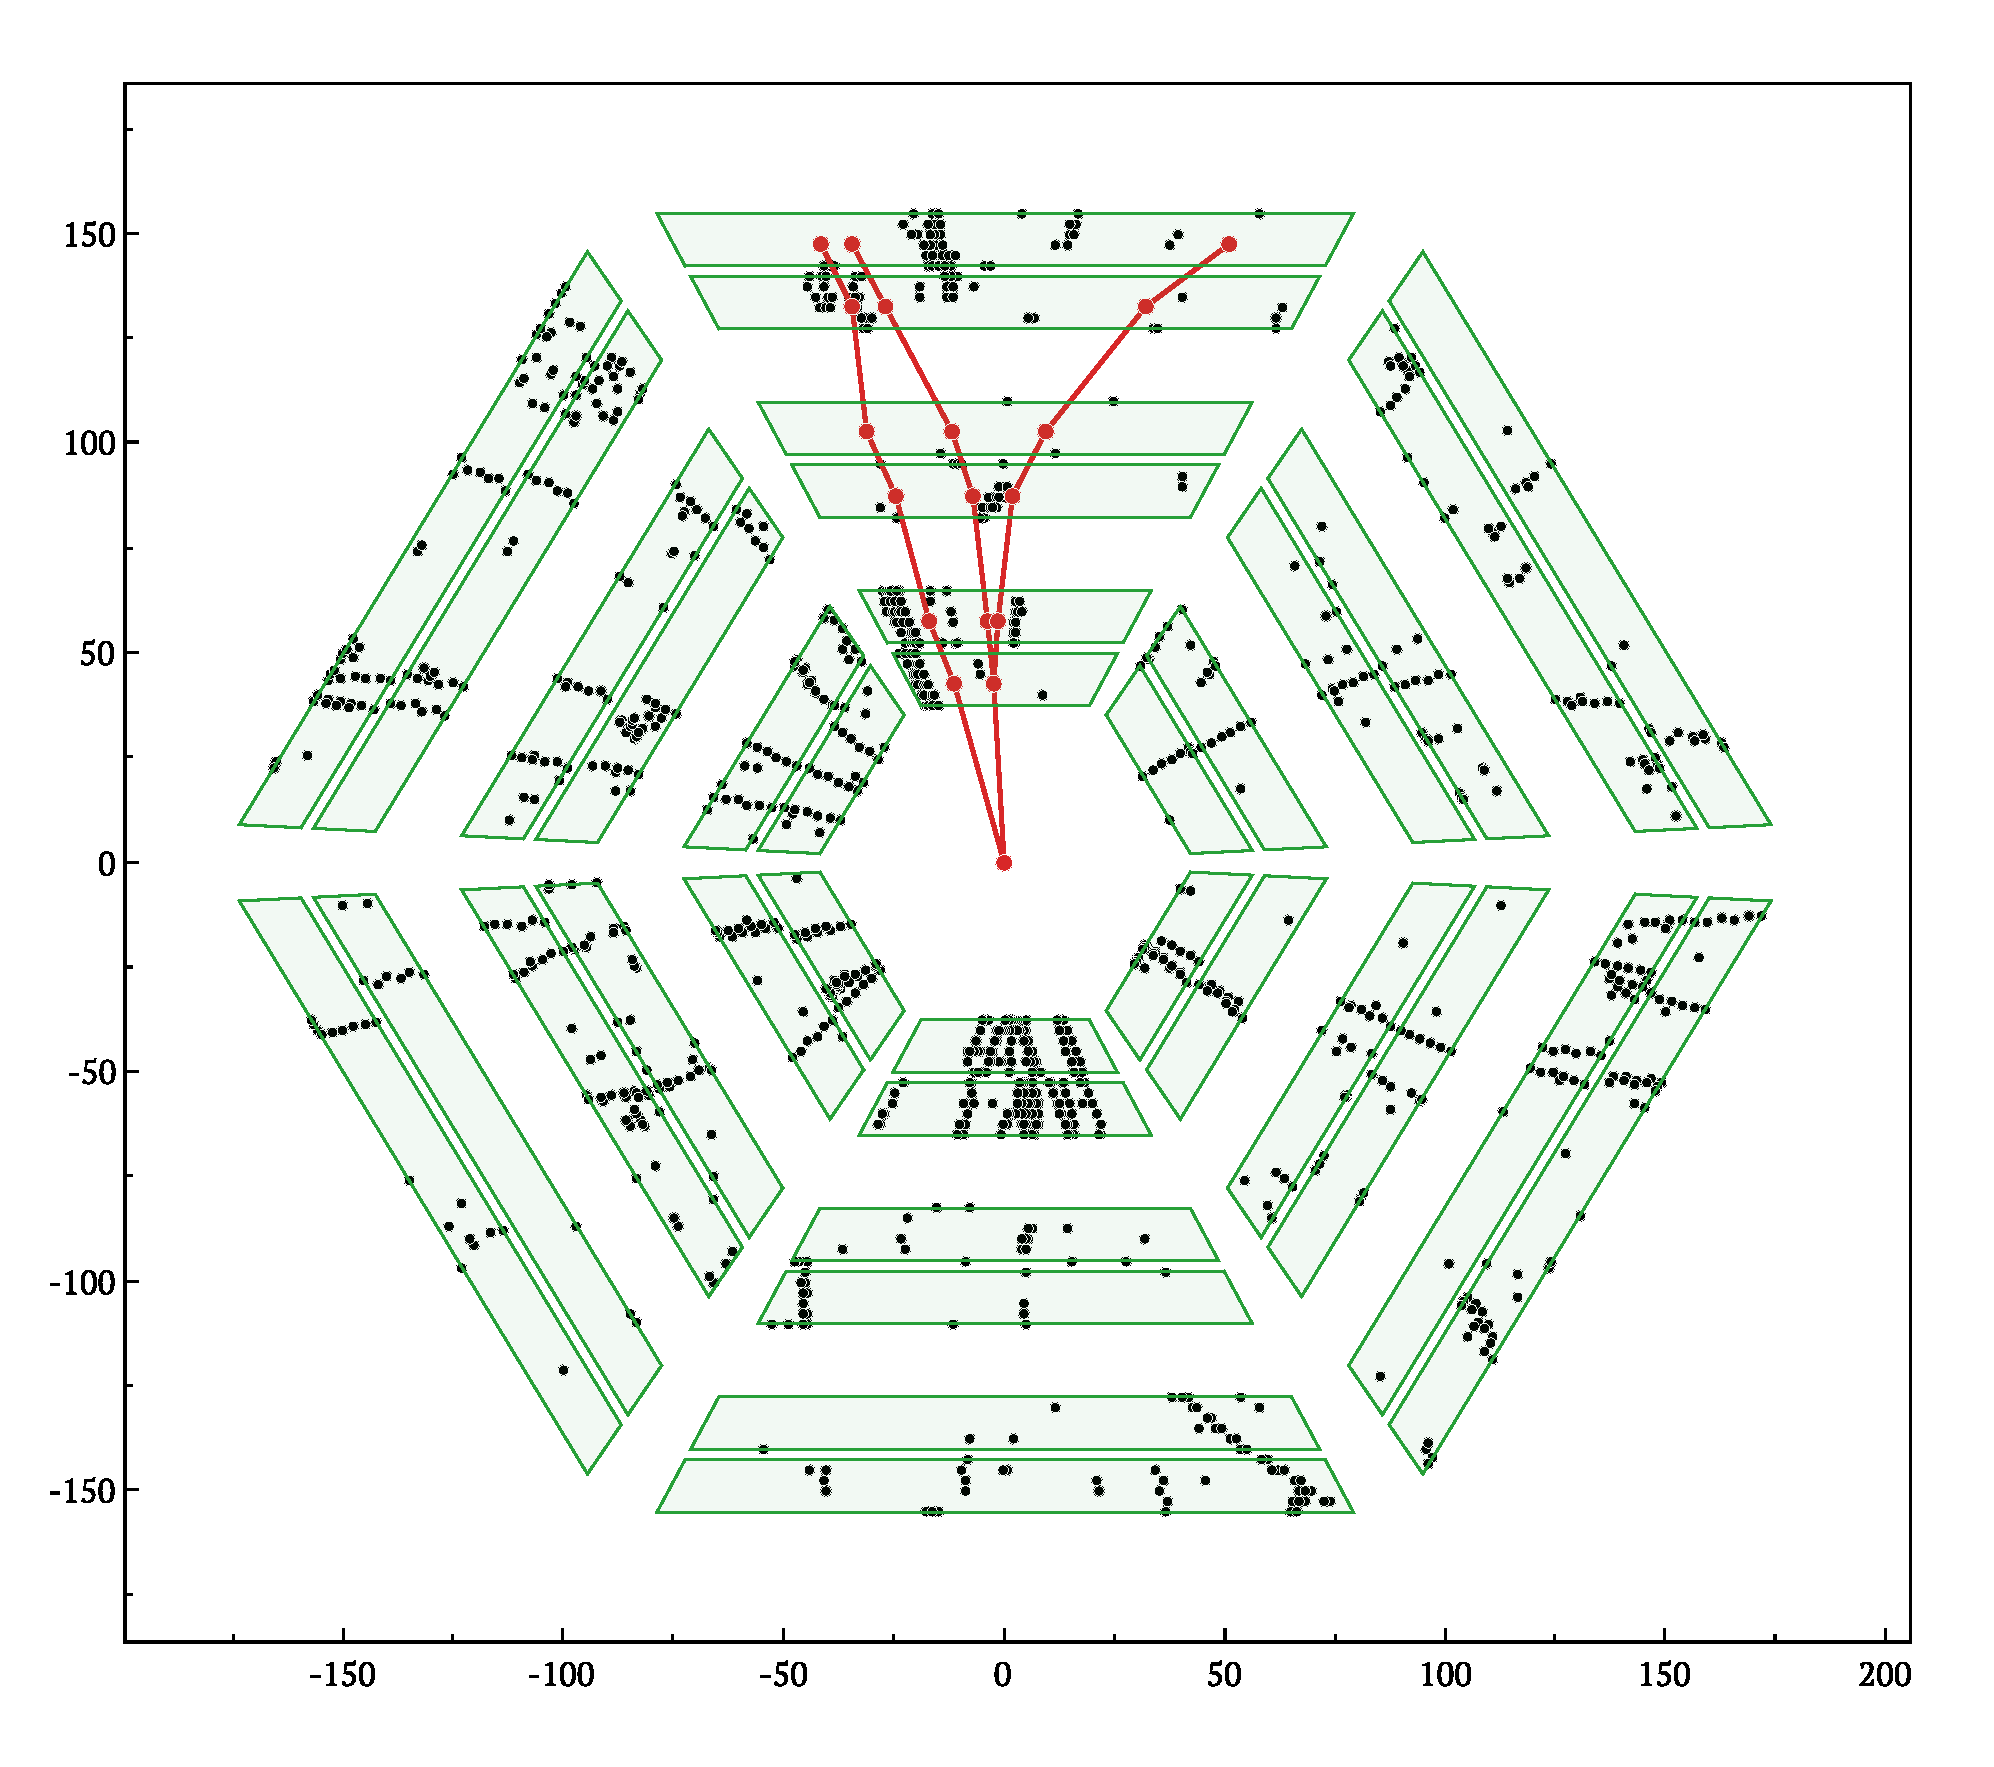
\includegraphics[width=0.32\columnwidth]{images/dc_example_view.pdf}
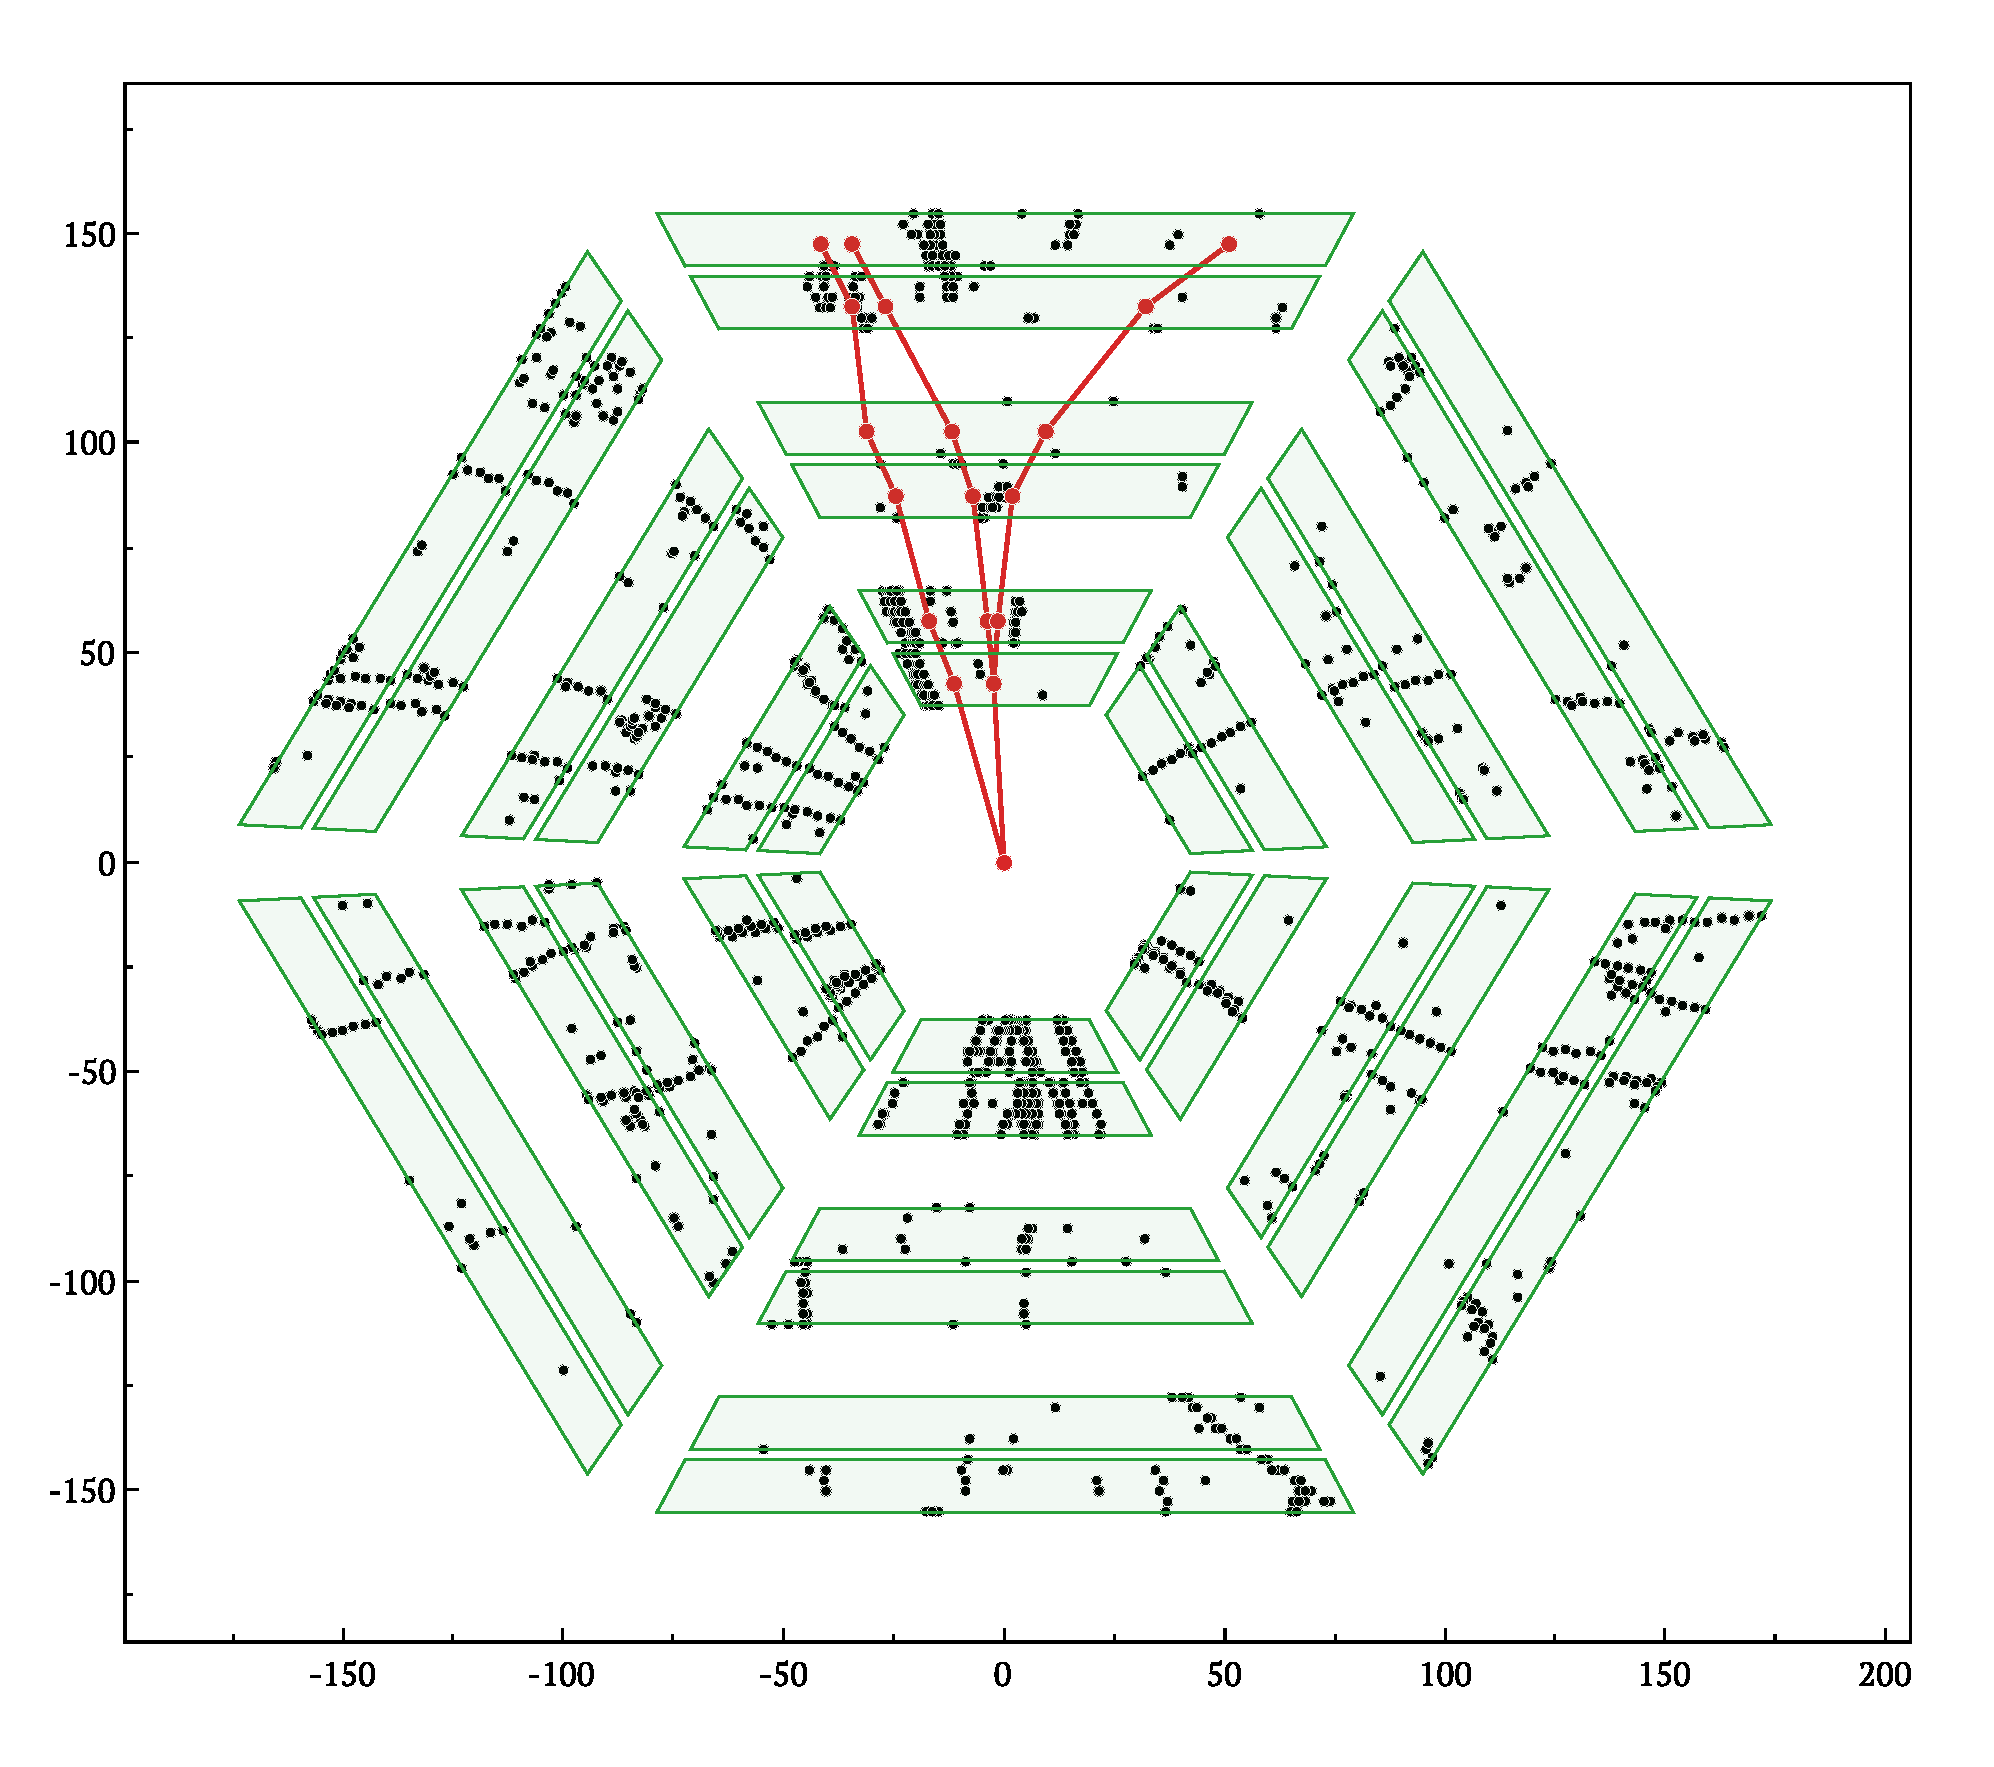
\includegraphics[width=0.32\columnwidth]{images/dc_example_view.pdf}
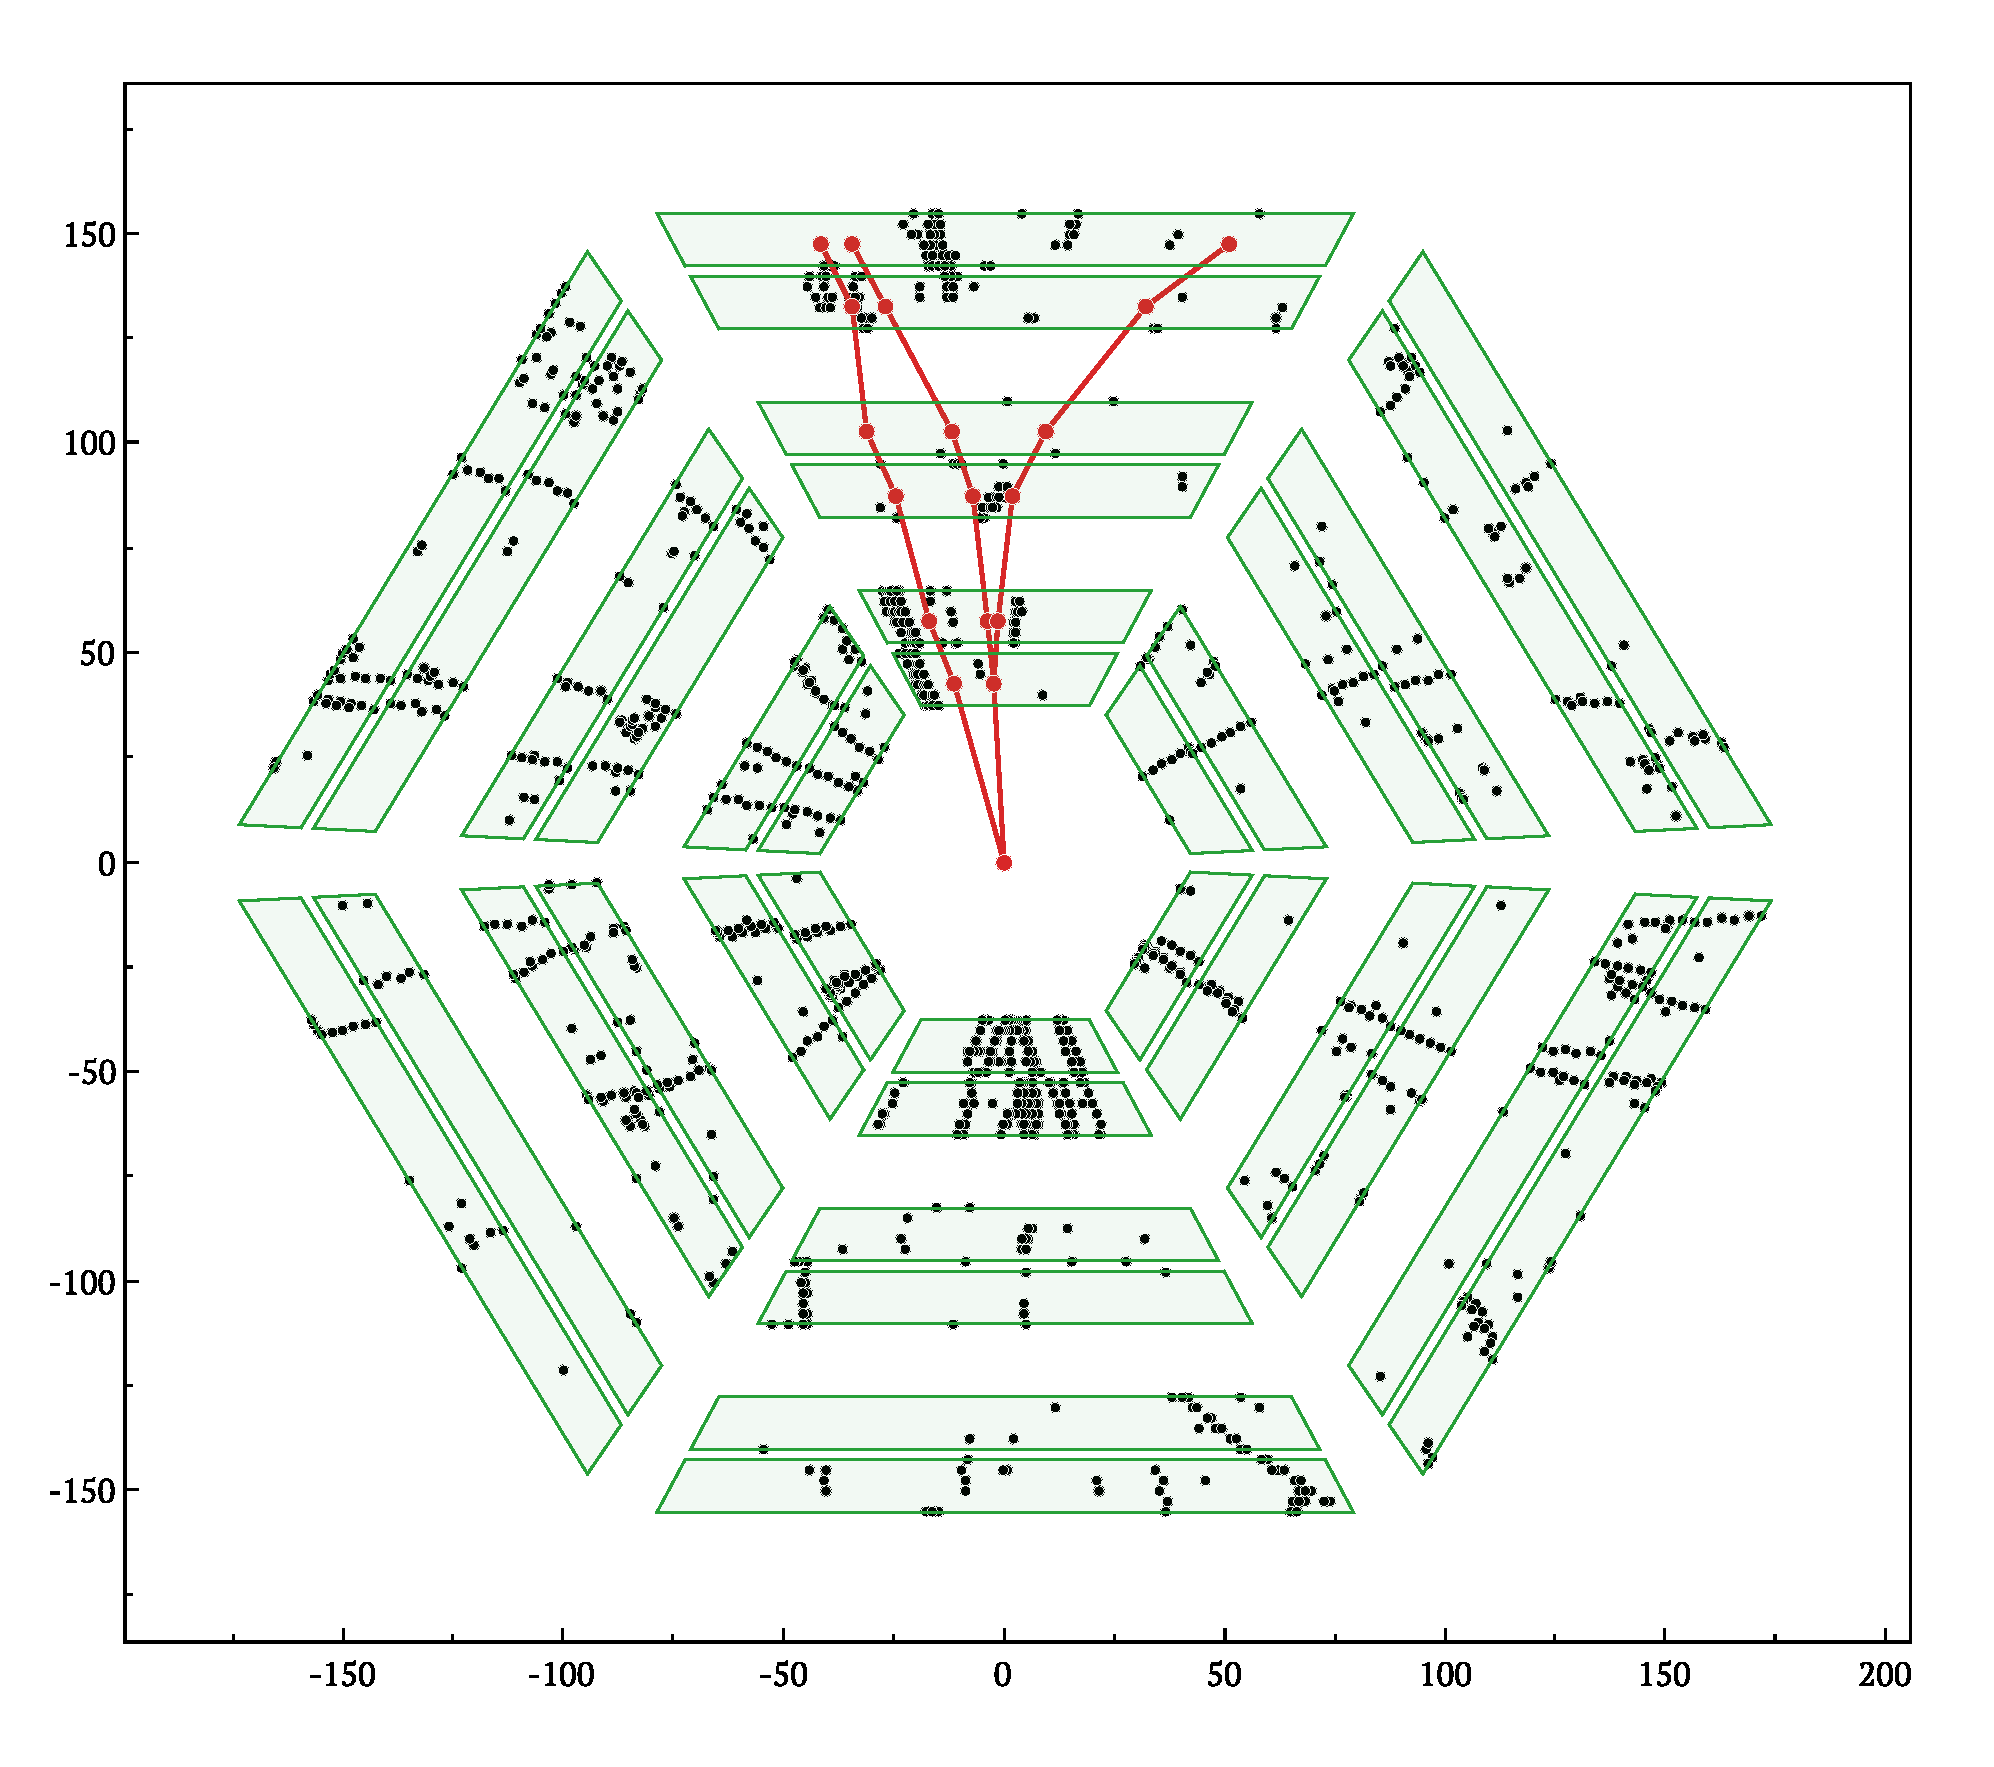
\includegraphics[width=0.32\columnwidth]{images/dc_example_view.pdf}
\caption{Example View for Drift Chambers (all 6 sectors). } 
\label{fig:CLAS12}
\end{figure}


\section{Acknowledgments}

This material is based upon work supported by the U.S. Department of Energy, Office of Science, Office of Nuclear Physics under contract DE-AC05-06OR23177, and
 %This research was sponsored in part from Jefferson Lab grant no. XXX, SURA grant No. CNF-19-04, 
 NSF grant no. CCF-1439079 and the Richard T. Cheng Endowment. This work was performed using the Turing and  Wahab computing clusters at Old Dominion University.
 
 \begin{thebibliography}{}
%
% and use \bibitem to create references.
%
\bibitem{Burkert:2020akg}
Burkert, V.D. and others, The CLAS12 Spectrometer at Jefferson Laboratory, Nucl. Instrum. Meth. A \textbf{959},163419 (2020)
% Format for Journal Reference
%Journal Author, Journal \textbf{Volume}, page numbers (year)
% Format for books
\bibitem{Mestayer:2020saf}
 "Mestayer, M.D. and others", The CLAS12 drift chamber system, Nucl. Instrum. Meth. A",\textbf{959} 163518 (2020)
\bibitem{Kalman1960}
  Kalman, R. E., A New Approach to Linear Filtering and Prediction Problems, Journal of Basic Engineering, \textbf{82}, 35-45 (1960)
\bibitem{Gavalian:2020oxg}
Gavalian, Gagik and Thomadakis, Polykarpos and Angelopoulos, Angelos and Ziegler, Veronique and Chrisochoides, Nikos, Using Artificial Intelligence for Particle Track Identification in CLAS12 Detector, \textbf{2008.12860}, (2020)
\bibitem{Gavalian:2020xmc}
 Gavalian Gagik,Auto-encoders for Track Reconstruction in Drift Chambers for CLAS12, \textbf{2009.05144}, (2020)
\bibitem{Thomadakis:2022zcd}
   Thomadakis, Polykarpos and Angelopoulos, Angelos and Gavalian, Gagik and Chrisochoides, Nikos, De-noising drift chambers in CLAS12 using convolutional autoencoders, \textbf{271}, 108201 (2022)
%\bibitem{RefB}
%Book Author, \textit{Book title} (Publisher, place, year) page numbers
% etc
\end{thebibliography}

%\newpage
%\bibliography{references}
%\bibliographystyle{ieeetr}

\end{document}
